% Boxes are to use reference like the main text, but the numbering should start after
% the last reference of the main text.
% Ergo, it makes sense in LaTeX to have the boxes after the main text...so we get
% the numbering right


\section{Box 1: Nonnegative sparse coding (NSC)}
\label{box:NSC}

% Need to keep it under 400 words

\Acf{NSC} combines \acf{NMF},
a linear dimensionality reduction technique from statistical learning,
with sparse population coding from neural network theory
\citep{Hoyer2002,EggertKorner2004}.
\ac{NMF} belongs to a class of methods that can be used to decompose
a multivariate data matrix \textbf{V}
into an inner product of two reduced-rand matrices \textbf{W} and \textbf{H}.
\ac{NMF} assumes that the observed data in \textbf{V} are caused by a collection
of latent factors weighted by nonnegative numbers,
representing both the presence and the intensity of the cause.

In the context of \ac{NSC},
\textbf{V} and \textbf{H} correspond to activation values
of two distinct neuronal populations,
which are connected to each other via synaptic weight values
in \textbf{W}
(Fig.~\ref{fig:NMF|reconstruction}).
Consider a number of data samples $s \in [1, S]$, for example,
in the form of observed firing rates of a population of $F$ neurons.
If we arrange the observed values of the $s$-th observation 
into a vector $\vec{v}_s$,
and if we arrange all vectors into the columns of a data matrix \textbf{V},
then linear decompositions describe these data as
$\mathbf{V} \approx \mathbf{WH}$.
Here, \textbf{W} is a matrix that contains as its columns
a total of $B$ \emph{basis vectors} of the decomposition, 
and \textbf{H} contains as its rows the \emph{hidden coefficients}
that give the contribution of each basis vector in the input vectors.
The difference between \textbf{V} and \textbf{WH} is termed
the \emph{reconstruction error}.

The goal of \ac{NSC} is then to find a linear decomposition of \textbf{V}
that minimizes the reconstruction error,
while guaranteeing that both \textbf{W} and \textbf{H} are sparse.
This can be achieved by minimizing the following cost function
\citep{Hoyer2002}:
\begin{equation}
\min_{\mathbf{W}, \mathbf{H}} \frac{1}{2} ||\mathbf{X} -\mathbf{WH}||^2 + \lambda \sum_{ij} f(\mathbf{H}_{ij}),
\end{equation}
subject to the constraints
$\forall ij: \mathbf{W}_{ij} \geq 0$, $\mathbf{H}_{ij} \geq 0$, and
$||\vec{w}_i|| = 1$, where $\vec{w}_i$ denotes the $i$th column of \textbf{W}.
Here, the left-hand term describes the reconstruction error, which can
be minimized with \ac{NMF},
and the right-hand term describes the sparseness of the decomposition.
The trade-off between sparseness and accurate reconstruction
is controlled by the parameter $\lambda$ ($\lambda \geq 0$), whereas
the form of $f$ defines how sparseness is measured
(a typical choice is the L1 norm on \textbf{H}).

Note that several modern implementations of the \ac{NMF} algorithm,
such as Matlab's \texttt{nnmf.m} function,
already implement sparsity constraints,
hence making \ac{NMF} indistinguishable from \ac{NSC}.


% %%%%%%%%%%%%%%%%%%%%%%%%%%%%%%%%%%%%%%%%%%%%%%%%%%%%%%%%%%%%%%%%%%%%%%%%%%% %

\section{Box 2: Equivalence of NMF to STDPH and neural mechanisms of NSC}
\label{Box:NMFvSTDPH}
% ELR: CLEANED UP STDP BOX.
% 398 WORDS TOTAL WHEN PASTED INTO WORD (INCLUDES CITATIONS, SO IS LIKELY SHORTER IN LATEX).

% First paragraph - STDP  on a single synapse
% Second paragraph - STDP on networks?
\jeffNote{This needs more details about the proof. In its present form, it mostly reviews STDP and homeostasis. I recommend expanding the third paragraph that starts with "We have shown that"}

\Acf{STDP} is a form of Hebbian learning in which synaptic weight changes
depend on the relative timing between pre- and post-synaptic spikes \citep{BiPoo1998,SongAbbott2000}. If pre-synaptic spike counts integrated over a critical window precede those of the post-synaptic neuron, then long-term potentiation (LTP) is induced, strengthening the weight. Otherwise, long-term depression (LTD) is induced, suppressing the weight. STDP is ubiquitous throughout the brain across the lifespan and can take on different forms \citep{Caporale2008STDP,Holtmaat2009STDP}. Simulations of \ac{STDP} can result in runaway feedforward excitation such that produces unrealistic firing rates. To obviate this problem in biology, the brain uses homeostatic mechanisms that modulate synaptic inputs and neuronal firing thresholds \citep{Watt2010}.

% One well-known homeostatic mechanism is synaptic scaling,
% wherein synaptic efficacy is regulated by neuronal activity
% to prevent runaway increases or decreases in synaptic strength.
We focus on synaptic scaling, a particular form of homeostasis which
multiplicatively scales weights up or down
depending on the average firing rate of the postsynaptic neuron, which has
been demonstrated to stabilize \ac{STDP} \citep{Carlson2013,Buonomano2005,VanRossum2000}.
We refer to this combination of \ac{STDP} and homeostatic synaptic scaling
as \ac{STDPH}.

% \mikeNote{I guess this paragraph should be tied to the figure I'm supposed to make}
% \krisNote{I referenced figure 2. It's tricky because I don't have room to describe why H and W are 1D (because we only have one output neuron).}

We have shown that, given a network with fewer output than input neurons and full connectivity from the input layer to the output layer, \ac{STDPH} iteratively acts to preserve the information in the first layer with the output layer neurons.
Given an input layer of neurons (represented by matrix \textbf{V}) connected to a single output layer neuron (represented by 
% \mikeNote{fixed vector notation}
row vector $\vec{h}^T$) we have proven that the \ac{STDPH} rule iteratively updates the synaptic weights in $\vec{w}$ in such a way as to minimize the reconstruction error of $|\mathbf{V} - \vec{w} \vec{h}^T|$, and that the \ac{NMF} update rule is mathematically equivalent to the \ac{STDPH} update rule \citep{Carlson2013}.

% \mikeNote{Is $\mathbf{wh^T}$ an outer product or should it be a vector \textbf{v}?}
% \krisNote{NMF Matrix question: $\mathbf{wh^T}$ is an outer product. Explanation:
% Let n = number of input 
% neurons, m = number of time steps, and r = number of output neurons. Let r = 1. Then, 
% $V$ is of dimensionality nxm, $w$ is of dimensionality nx1 (column vector), and $h^T$
% is of dimensionality 1xm (row vector). The problem is I was not consistent with what I
% told you for conventions. I have used bold capital for matrix, bold lower case for column,
% and bold columm transpose for row.}


% \mikeNote{I said this in the main text}
% The equivalence of \ac{STDPH} to \ac{NMF} should not come as a particular surprise and in fact
% their similarities were alluded to \citep{Masquelier2010} before the mathematical proof for the
% single neuron case \citep{Carlson2013}.
% The equivalence of \ac{STDPH} to \ac{NMF} can be viewed as analogous to the equivalence of Oja\textsc{\char13}s rule to \ac{PCA} in the following way.
% Oja\textsc{\char13}s rule was developed to stabilize the rate-based Hebbian learning rule
% by introducing multiplicative normalization
% just as homeostatic synaptic scaling was added to \ac{STDP}
% for stabilization \citep{Oja1982}.

% Emily note to self: I already mention this a couple places so I can either work it in or replace it elsewhere
% \krisNote{Although relevant, I'm not sure we'll have room for these two sentences}
% As mentioned in Box 1, \ac{NSC} combines the dimensionality reduction of \ac{NMF}
% with the concept of sparse population codes from neural network theory
% \citep{Hoyer2002,EggertKorner2004}.
% \ac{NSC} can be viewed as an additional constraint on \ac{NMF},
% requiring sparsity in the neural firing, represented in the $\mathbf{h}$ vector.
% Third paragraph can be WTA/lateral inhibition.

To induce sparsity in networks of neurons, there must be a mechanism that causes each output layer to learn a different component of the total information represented by the input layer \citep{Foldiak1990}, which may be achieved by competition among units. Lateral or feedforward inhibition is often used to induce competition in SNNs, since it offers a biologically plausible mechanism to implement a \ac{WTA} architecture \citep{Coultrip1992}, although other groups have suggested that thresholding can also achieve sparse codes \citep{Rozell2008}. Therefore, \ac{NSC} can be attained in a two-layer network with \ac{STDPH} and a \ac{WTA} architecture via inhibitory connections within or between layers. Interestingly, popular implementations of \ac{NMF} (e.g., MATLAB, Scikit-Learn) include a constraint on the L1 norm of \textbf{H} that automatically lead to sparsity. Alternatively, an explicit sparsity level can be incorporated into models of \ac{NMF}, such as in Hoyer\textsc{\char13}s model \citep{Hoyer2004}.

%%%%%%%%%%%%%%%%%%%%%%%%%%%%%%%%%%%%%%%%%%%%%%%%%%%%
% Methods for EA experiments of RSC. This is too long (~470 words).

\section{Box 3: Evolutionary Algorithm and SNN Evaluation}
\label{box:EA}
% \mikeNote{Slightly reworded things. This allowed removal of crossover and mutation from Glossary. Fitness is explained well here, too - might not need a Glossary entry either.}
Evolutionary algorithms are a class of optimization algorithms loosely based on concepts from evolution. A set of individuals (in this case, \acp{SNN}) have a set of parameters to be evolved, which are initialized for the first generation with size $N$. The population undergoes a training and a testing phase followed by evaluation as determined through a user-defined function that measures how well individuals in the population meet the desired criteria. The resulting value is the individual's level of \emph{fitness}.
A certain number of individuals are then chosen as parents for the next generation,
which can undergo \emph{crossover}
(i.e., where a child inherits parameters from its parents whose values
have been swapped at random)
and/or \emph{mutation}
(i.e., where a child inherits parameters from its parents with values
randomly chosen from a distribution of values)
to produce a new generation of individuals.
This process continues until the fitness of the population no longer improves.

Carlson and colleagues \citep{Carlson2014}
developed an automated tuning framework
that incorporates a plugin to CARLsim \citep{BeyelerCarlsonChou2015}
for running evolutionary algorithms using the ECJ library \citep{white2012}.
The plugin is used to pass information about the \ac{SNN} population
(e.g., number of generations to run, parameters to be evolved and their ranges,
mutation and crossover rates)
back and forth between CARLsim and ECJ (Fig.~\ref{fig:CarlsimECJ}).
The networks in the population are created, trained, tested, and evaluated using CARLsim.
The resulting fitness scores for each individual in the population 
are then handed off to ECJ,
which determines the parameters for the next generation according to
the selection criteria defined in the parameter file,
and the cycle repeats.

\begin{figure}[h]
	\centering
	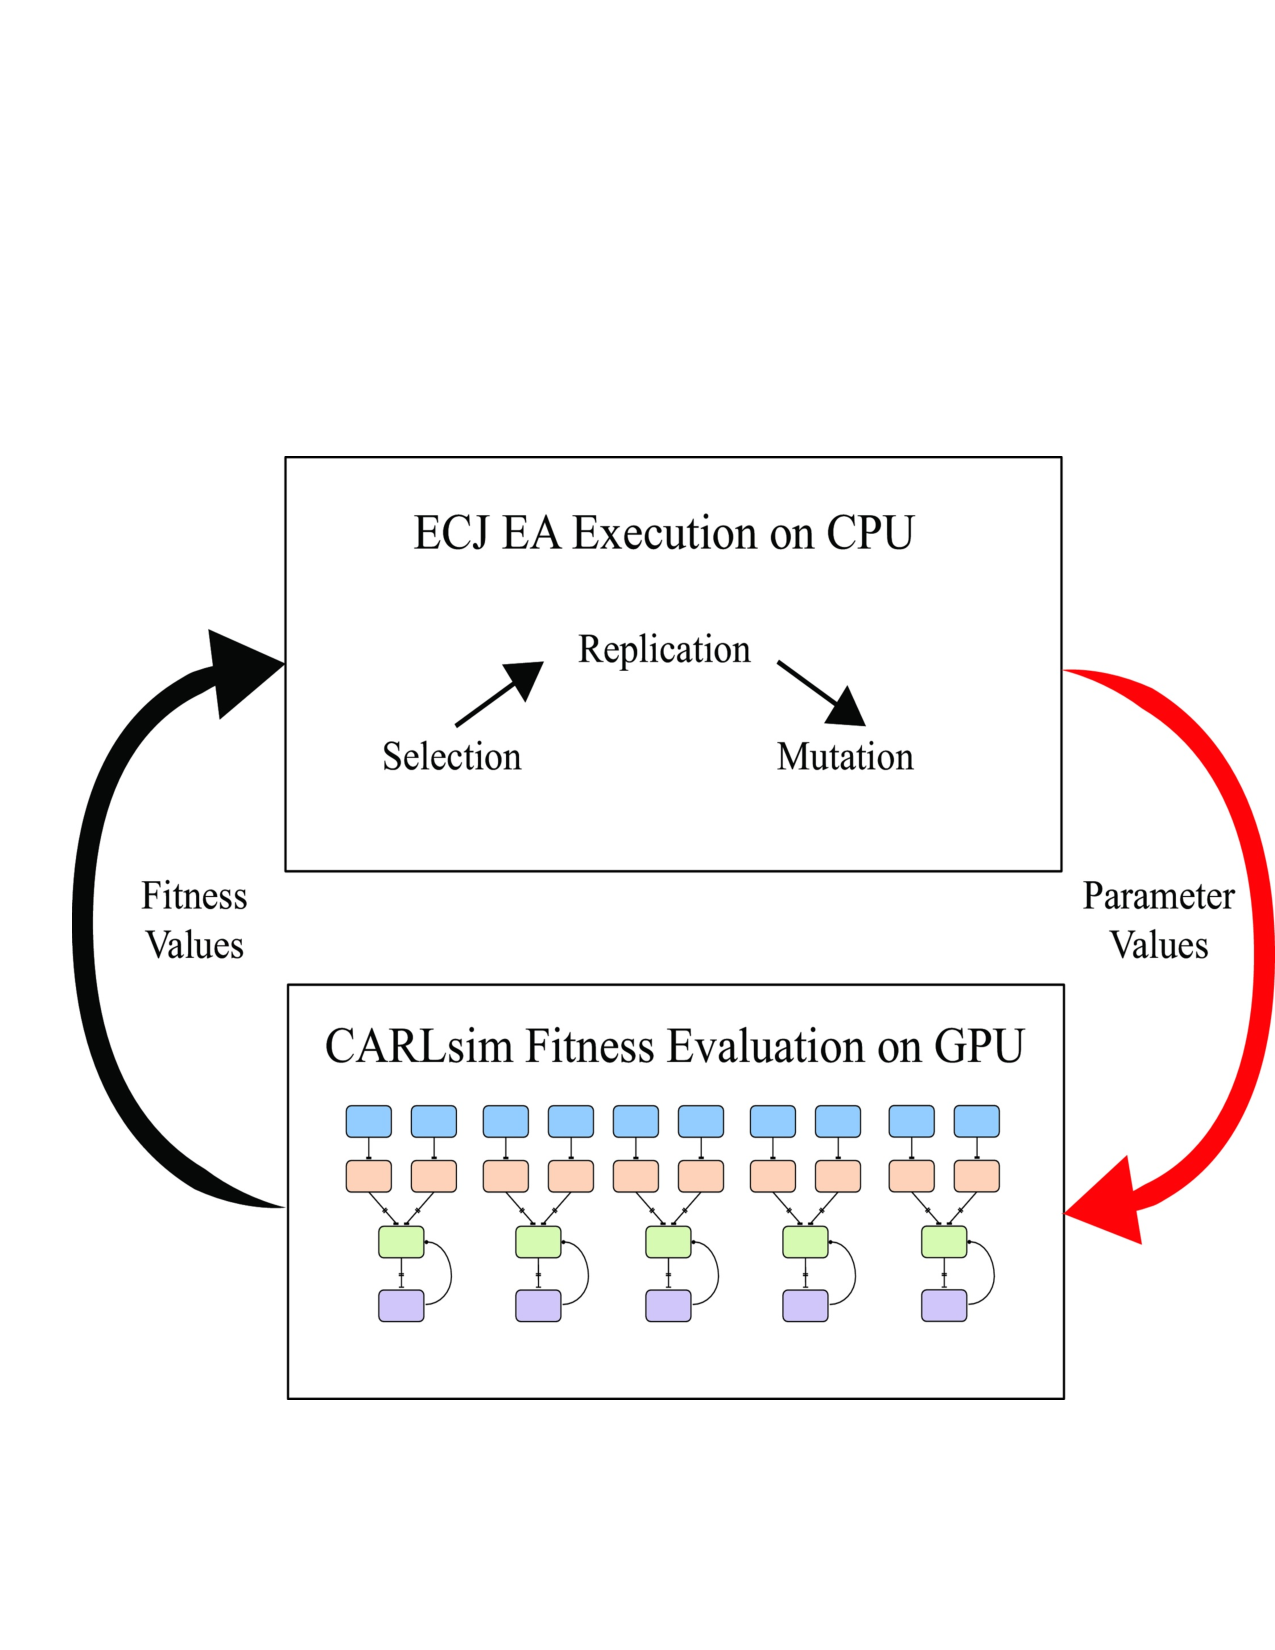
\includegraphics[scale=.8]{CarlsimECJ}
    \caption{CARLsim-ECJ pipeline for evolving \acp{SNN} using ECJ
    (adapted from \citep{Carlson2014}).
    ECJ is used to initialize the parameters being tuned, which are passed to CARLsim and used to set the parameters of each network in the population of \acp{SNN} (red arrow). The \acp{SNN} are initialized, run, and evaluated using CARLsim. Following fitness evaluation using some user-defined criteria, the resulting fitness values for each individual in the population are sent to ECJ (black arrow). ECJ chooses parents from the population and performs selection, replication, and mutation on the parameters of the parent individuals in order to initialize the next generation of \acp{SNN}. This continues for a user-defined number of runs or until convergence.}
	\label{fig:CarlsimECJ}
\end{figure}

 In the experiments in which \acp{SNN} were used to replicate neurophysiological data, the evolutionary algorithm was used to optimize STDPH parameters in the model, corresponding to the temporal window over which spike times were integrated, the amount each synaptic weight increased or decreased, the initial weight range of each group of synaptic connections, and the target baseline firing rates of excitatory and inhibitory neurons. During each generation of the evolutionary run, models were trained on trials randomly selected from half of the available dataset, then tested on trials randomly selected from the latter half reserved for testing. At the end of each generation, synthetic neural activity was correlated with electrophysiologically recorded neural activity, which served as the fitness metric for the algorithm. After the model finished an evolutionary run, SNN activity closely matched the electrophysiological activity.
 
 
% This Drugowitsch paper seems highly relevant:
% Causal Inference and Explaining Away in a Spiking Network
% Rubén Moreno-Bote \& Jan Drugowitsch, Scientific Reports
% \url{https://www.nature.com/articles/srep17531}

% The spike-based implementation can be interpreted as a noisy
% version of the rate-based network (can it?)
